\chapter{User Interface Design}
<<<<<<< HEAD
In this chapter we discuss in detail the design of the User eXperience by the \emph{UX Diagram} and some mock-ups. The main intention during this stage of the project has been to extremely simplify the interactions between the user and the system, trying to guarantee the most intuitive and smooth experience. 
\\The first page the user will interact with is the Home Page obviously, from this point it is possible to log in or sign up into the system and also see a description of the main features of the \emph{Travlendar+} application.
Immediately after the log in phase the user will be redirected to his personal page. Here, he can perform several actions, such as: 
\begin{itemize}
    \item See the scheduled tasks
    \item See a detailed description of the current day schedule
    \item Have access to both the sharing based services and the public transport services 
    \item Add a new task
    \item Select a task to modify it or to simply look at more detailed information about it
    \item Change the global preferences
    \item See his profile
    \item Change the calendar granularity (by day, week, month)
    \item Log out from the system 
\end{itemize}  
In particular, when the user wants to start create a new task a pop up will be displayed and will ask the user to fill a number of fields to better detail the new task. A similar approach will be used to manage the selection and modification of a task.
On the other hand, when the user wants to have access to global preferences a new page will be displayed where all the travel related preferences might be modified. 
Finally, when the user wants to buy a bus ticket or rent a shared based vehicle it will be redirected to the appropriate web page or application by mean of a button. 
=======
>>>>>>> ad258dd7c9a37861a484c05c0be22fc9761a519f

\begin{figure}[H]
    \centering
    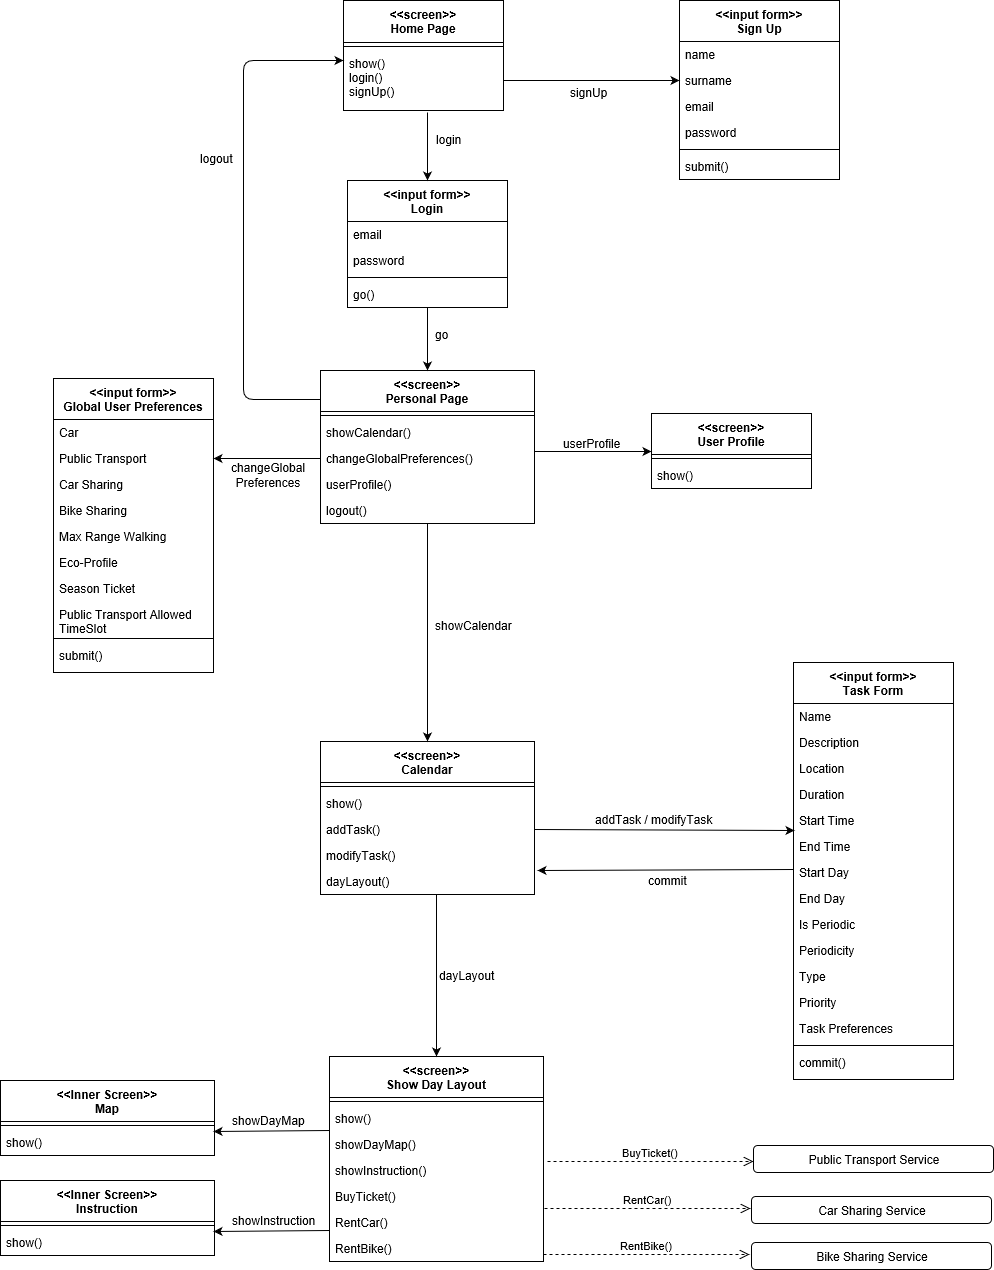
\includegraphics[scale=0.4]{Pictures/UXDiagram/UXDiagram.png}
    \caption{UX Diagram}
<<<<<<< HEAD
\end{figure}

As the reader may notice, the two pictures below represent a possible mock ups for the Home Page and the Sign Up screen.

\begin{figure}[H]
    \centering
    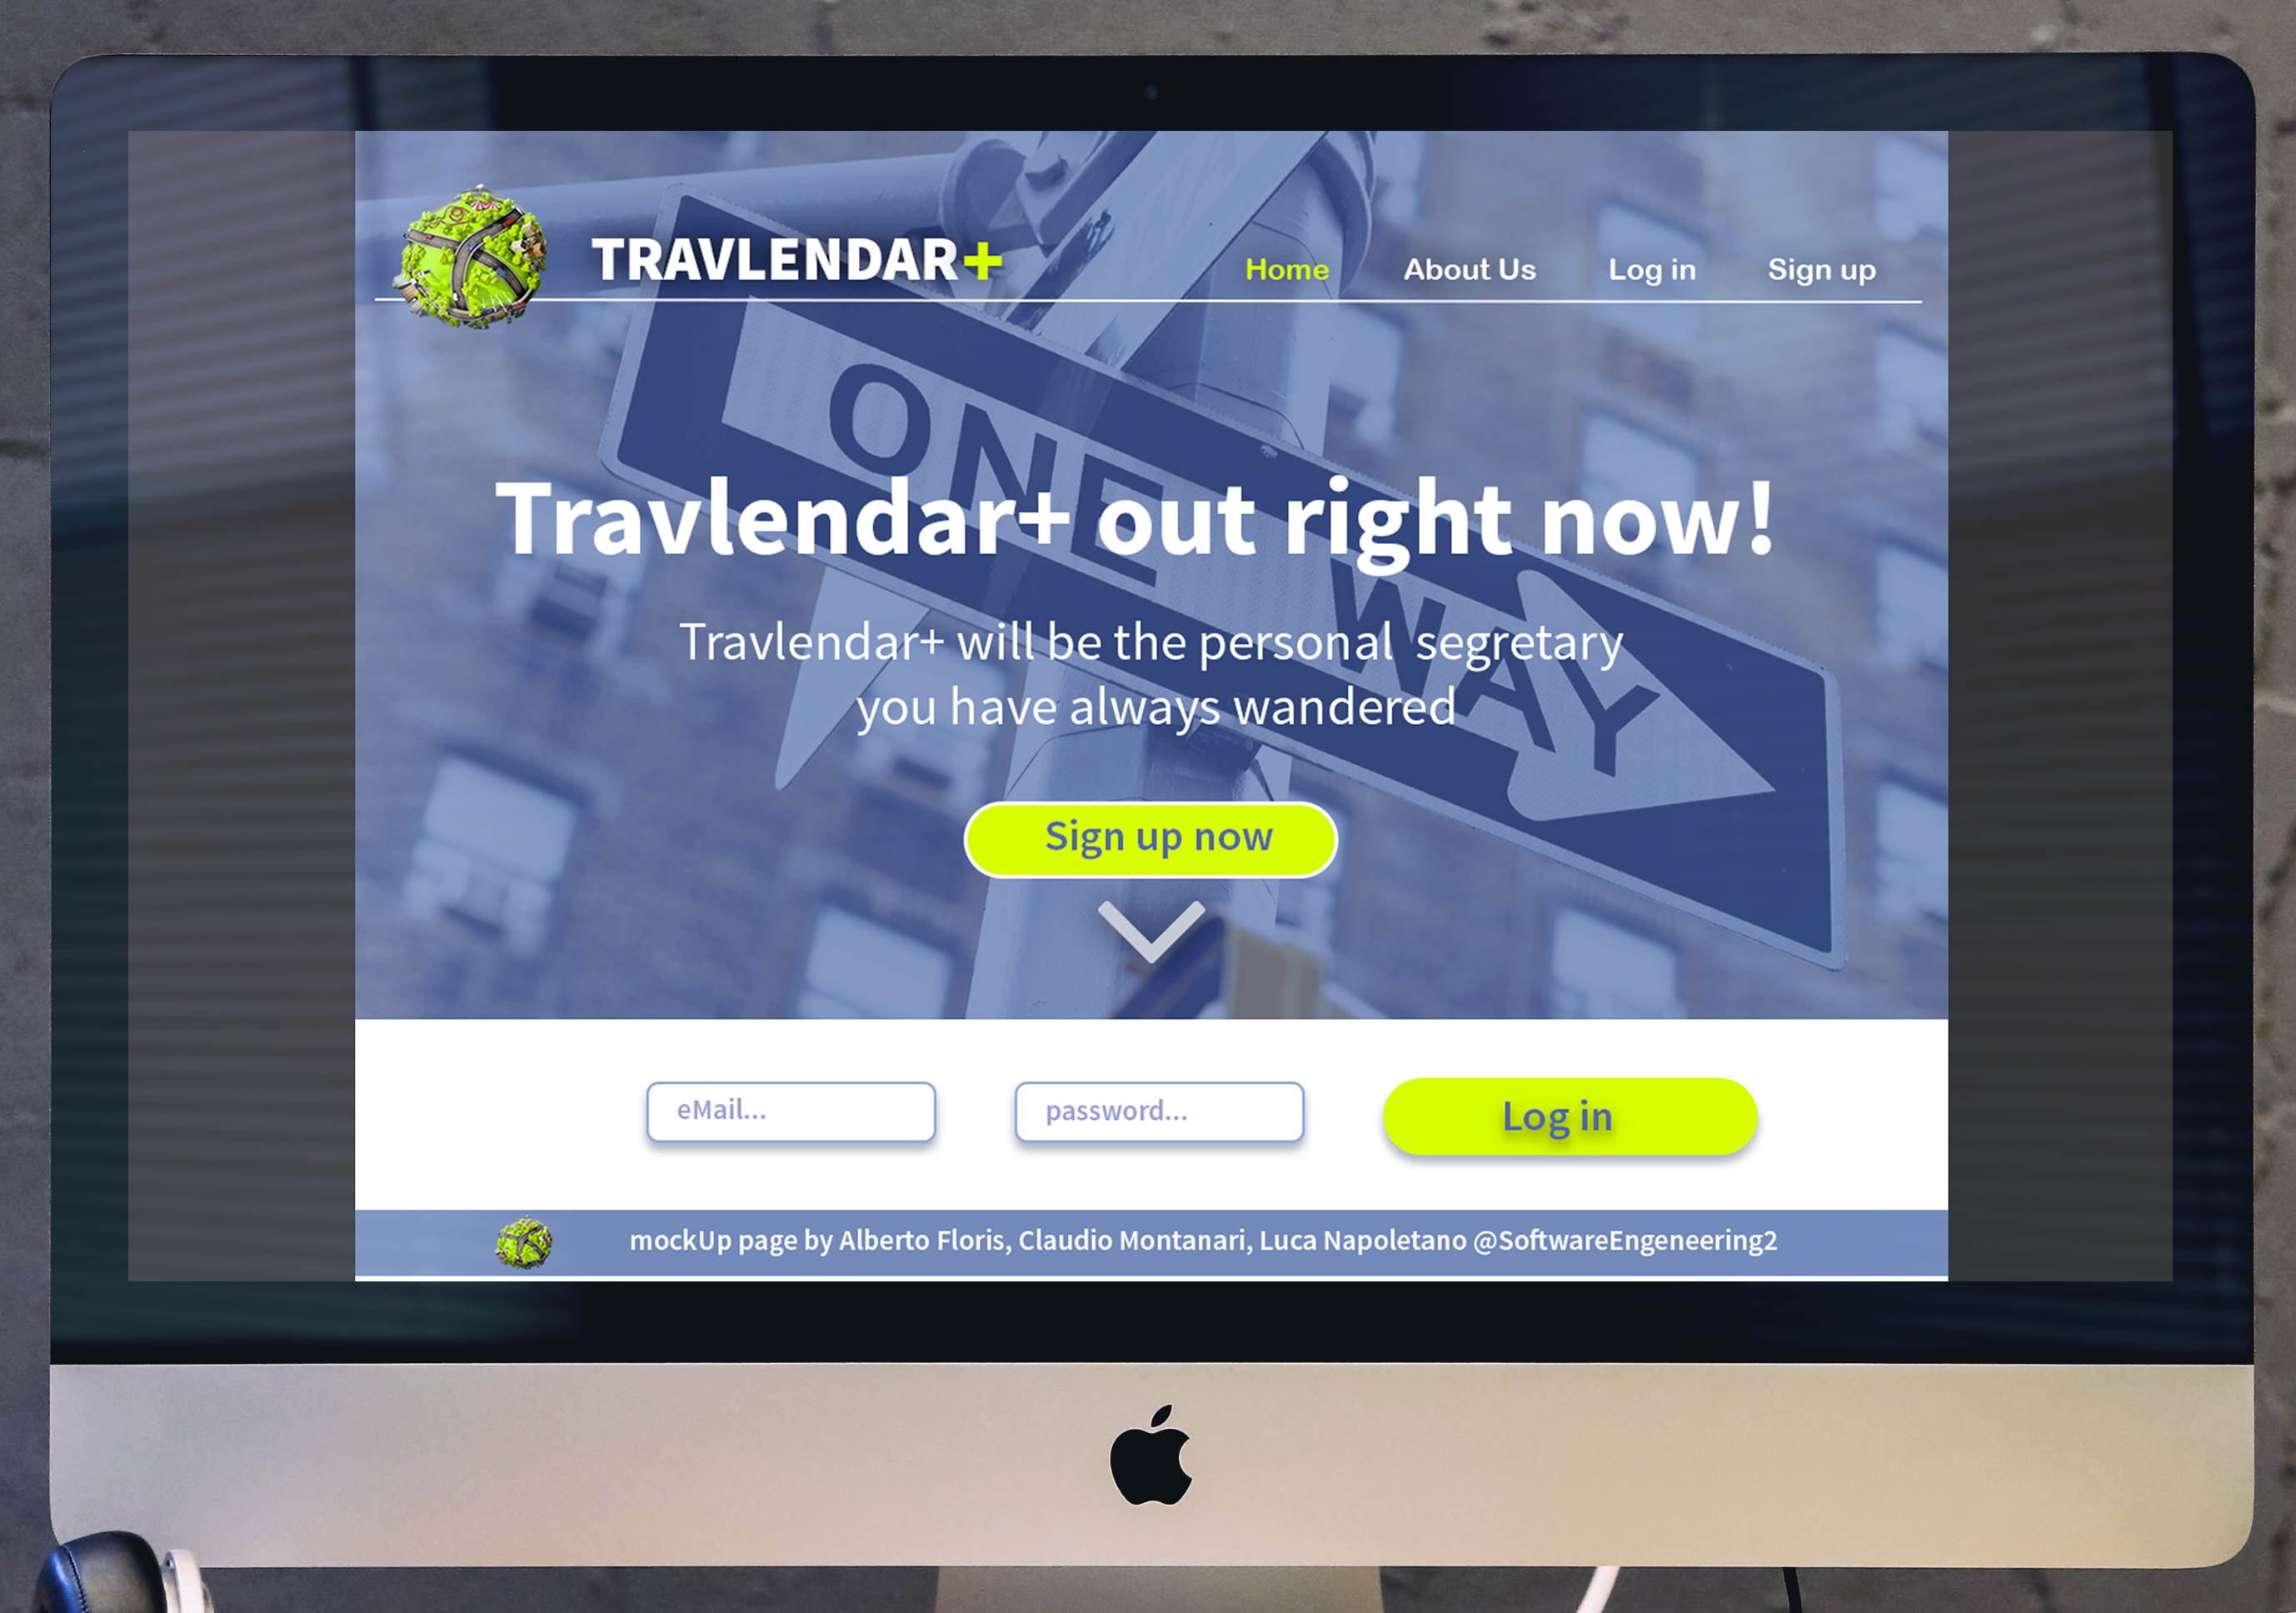
\includegraphics[scale=0.2]{Pictures/UXDiagram/desktopMockUpHome.png}
    \caption{Mock Up for the Home page of the \emph{Travlendar+} application}
    \label{fig:homePageMockUp}
\end{figure}

\begin{figure}[H]
    \centering
    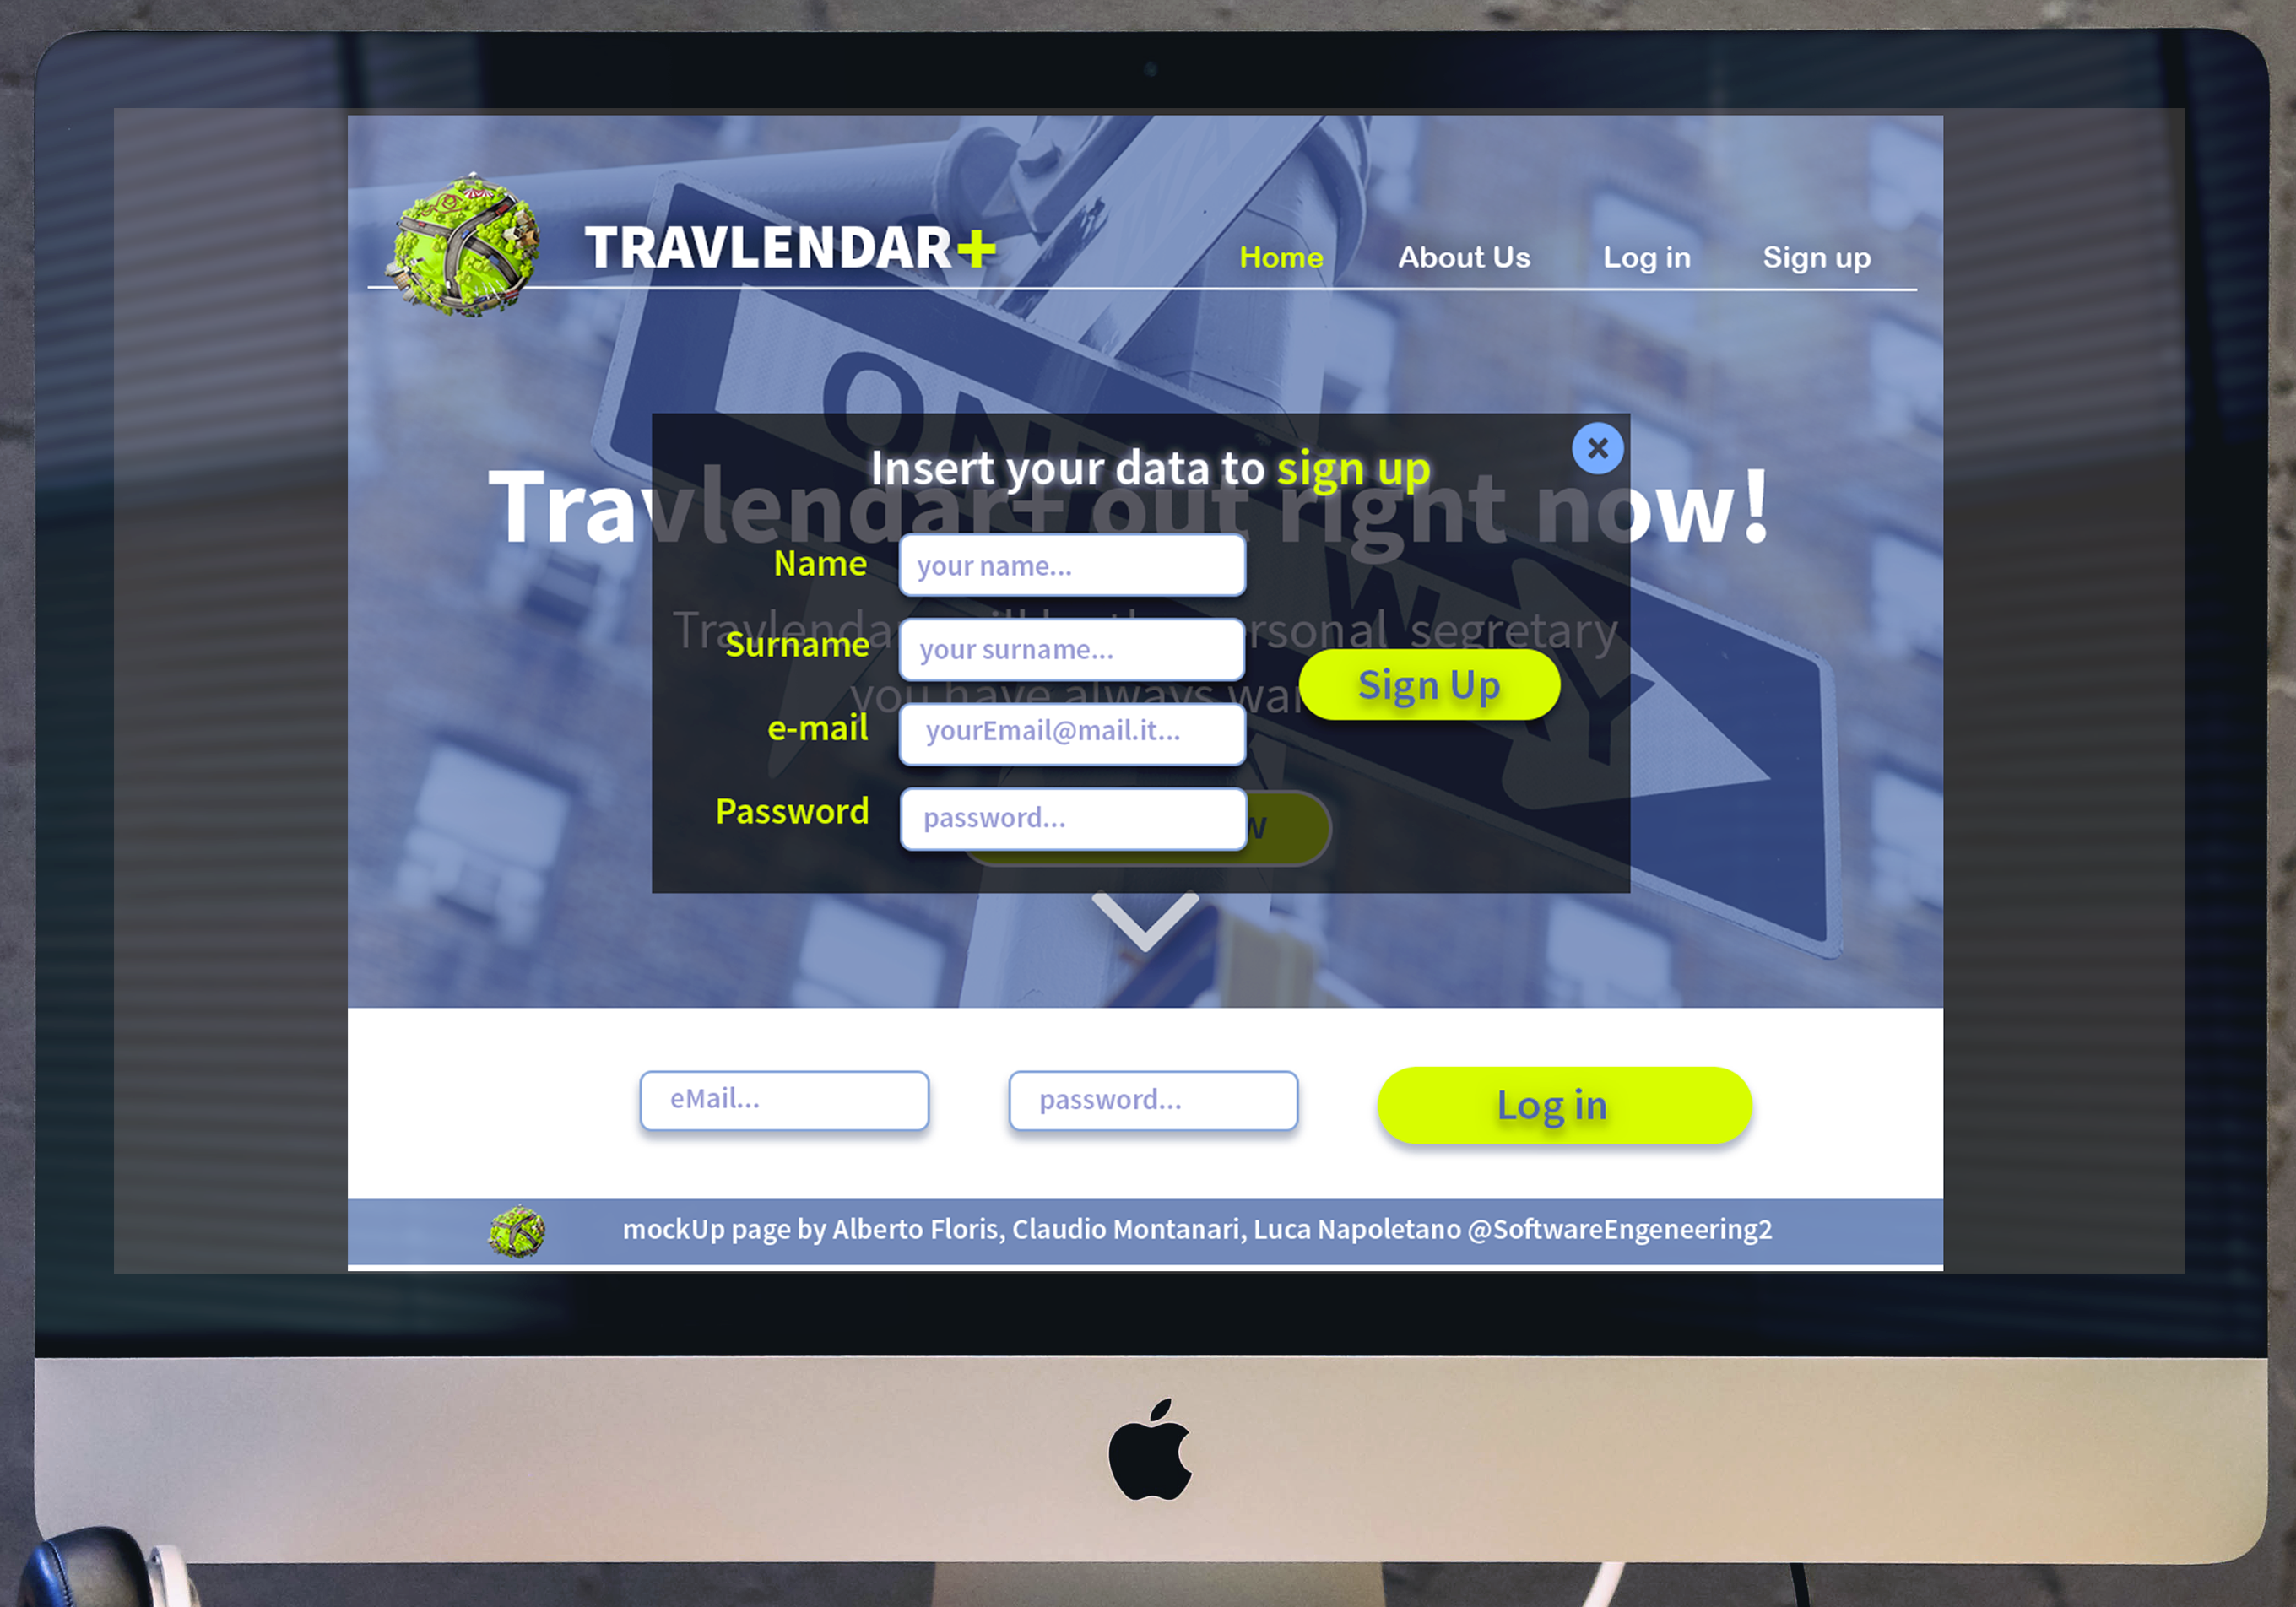
\includegraphics[scale=0.2]{Pictures/UXDiagram/desktopMockUpSignIn.png}
    \caption{Mock Up for the Sign Up screen}
    \label{fig:my_label}
\end{figure}

The two pictures below instead, stand for the user Calendar Page. In the left part of the screen the user has a summary of the current day schedule enriched by two buttons that stands for maps directions and vehicle or ticket services. \\On the right part is placed the calendar and just above the calendar the user has a menu bar for controlling the calendar layout, adding a task, change global preferences or log out of the system. 

\begin{figure}[H]
    \centering
    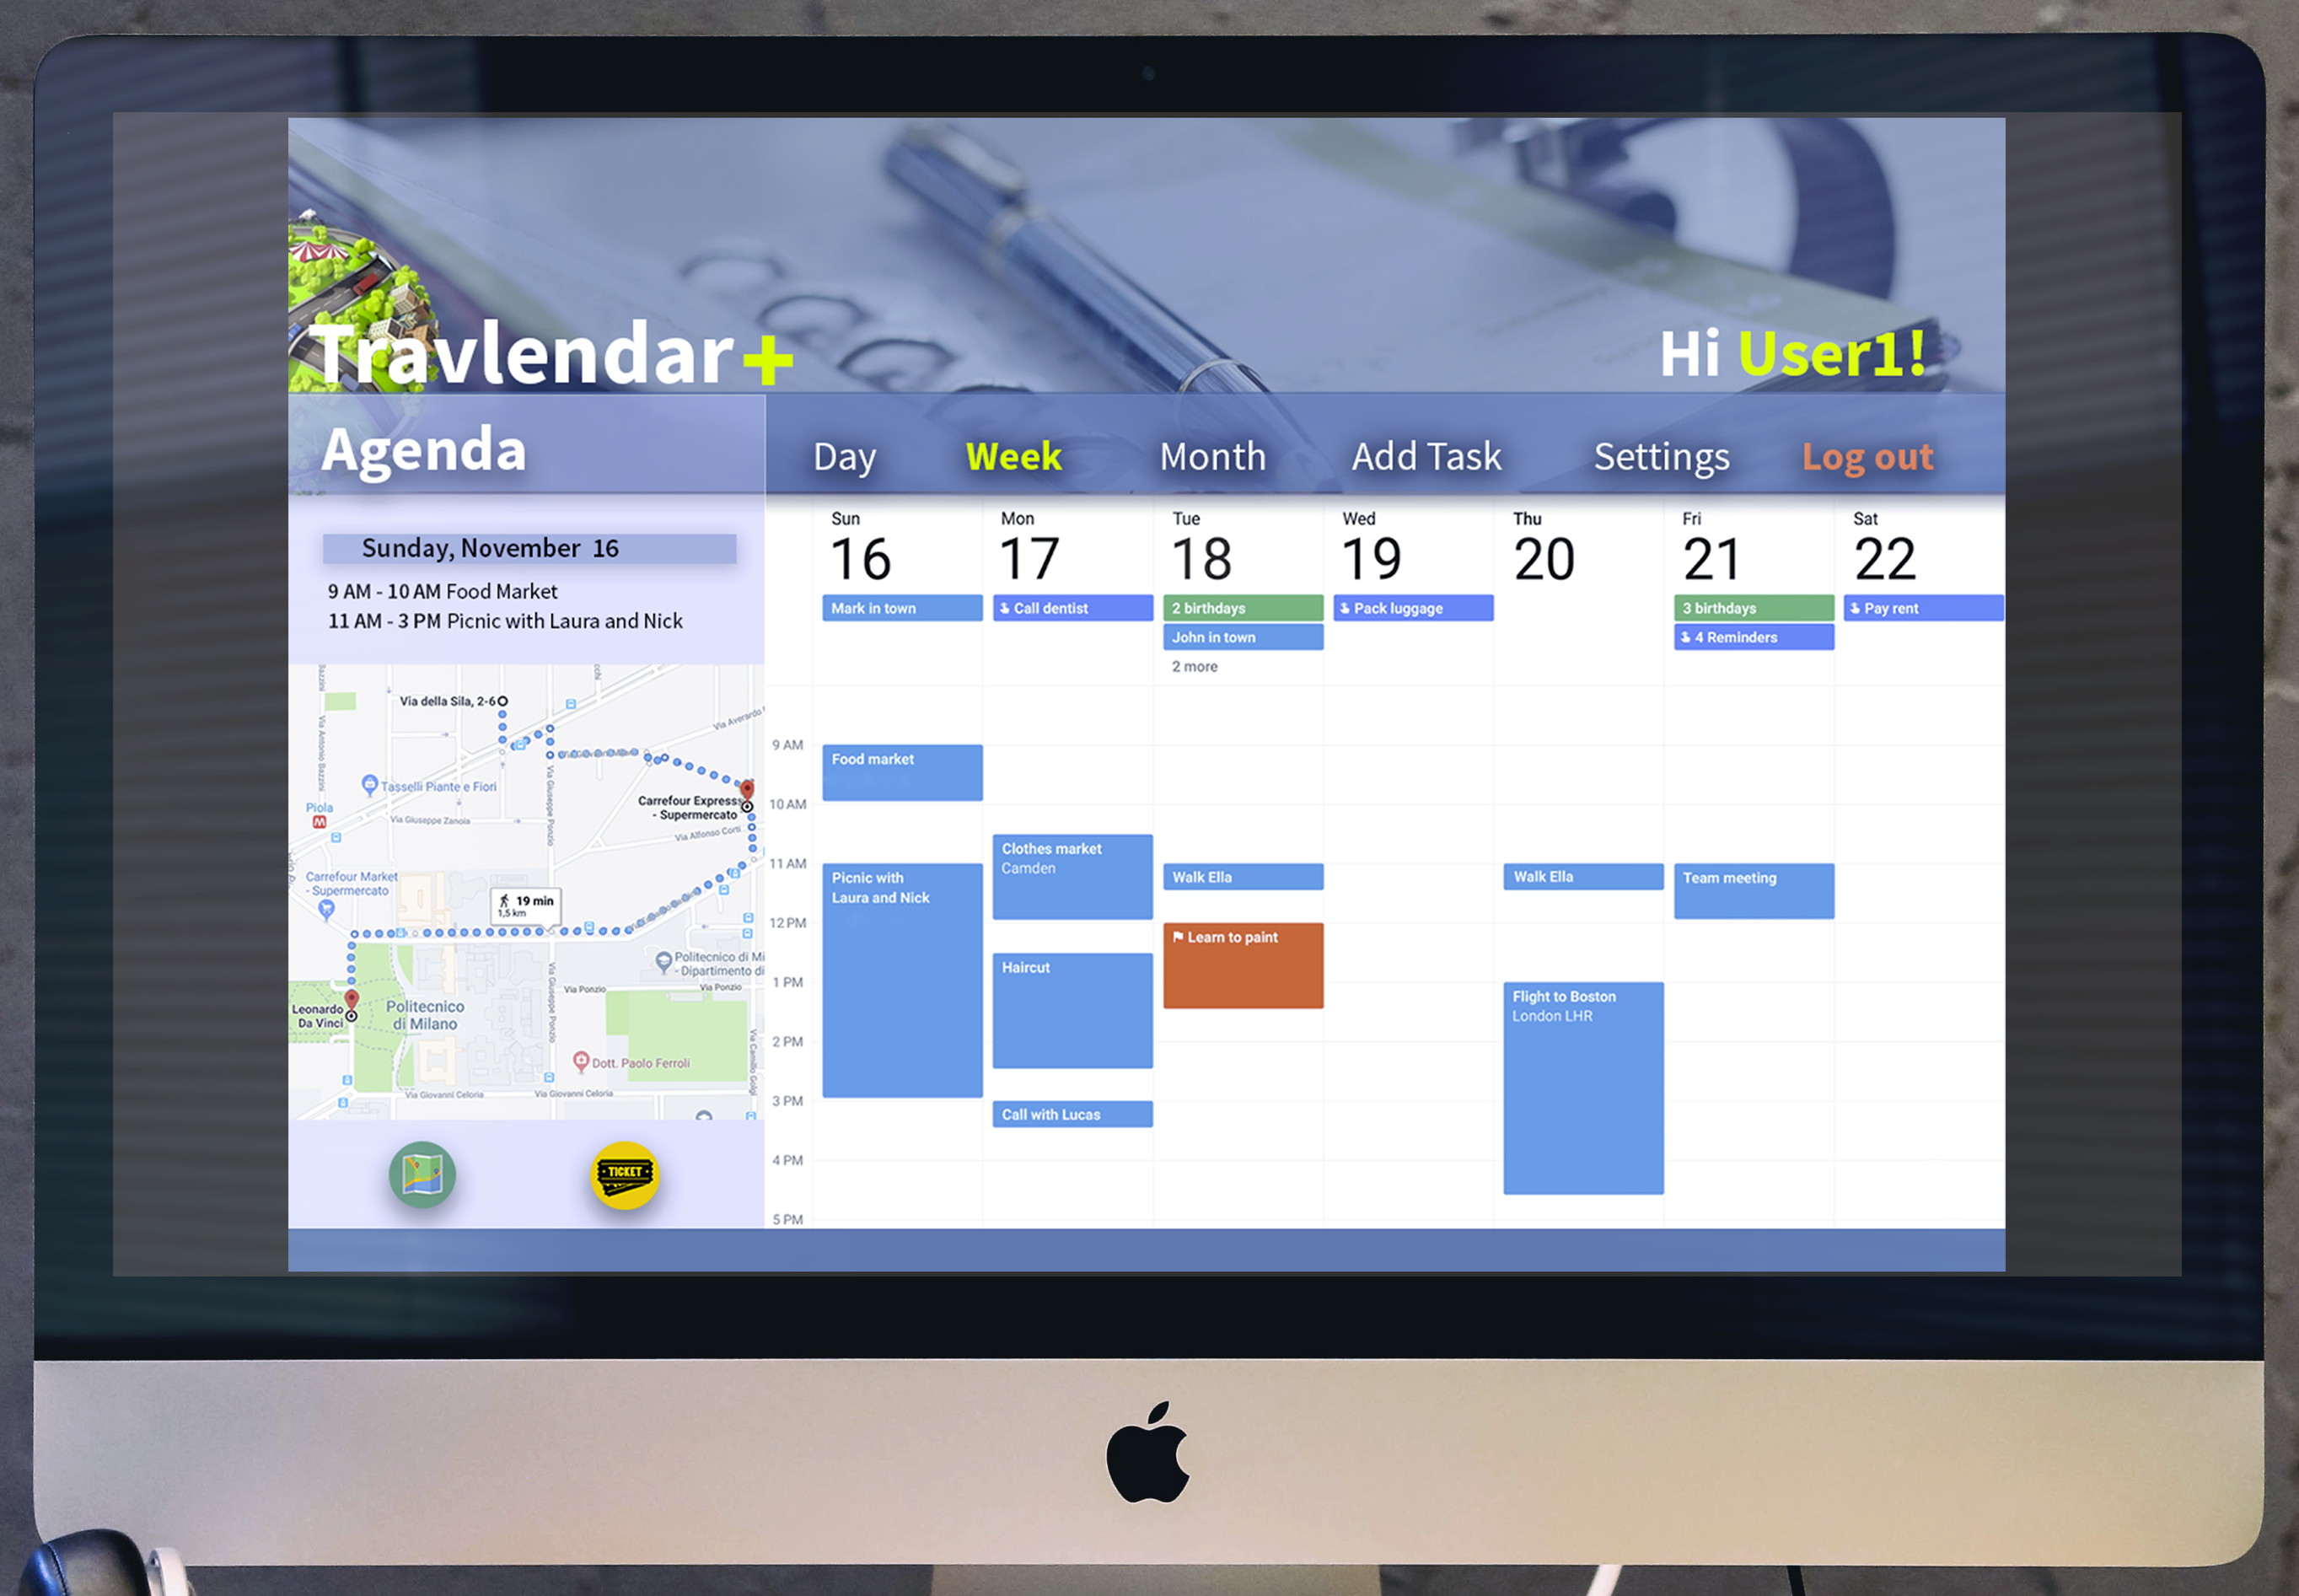
\includegraphics[scale=0.2]{Pictures/UXDiagram/desktopMockUpCalendar.png}
    \caption{Mock Up for the Calendar page}
    \label{fig:calendarMockUp}
\end{figure}

\begin{figure}[H]
    \centering
    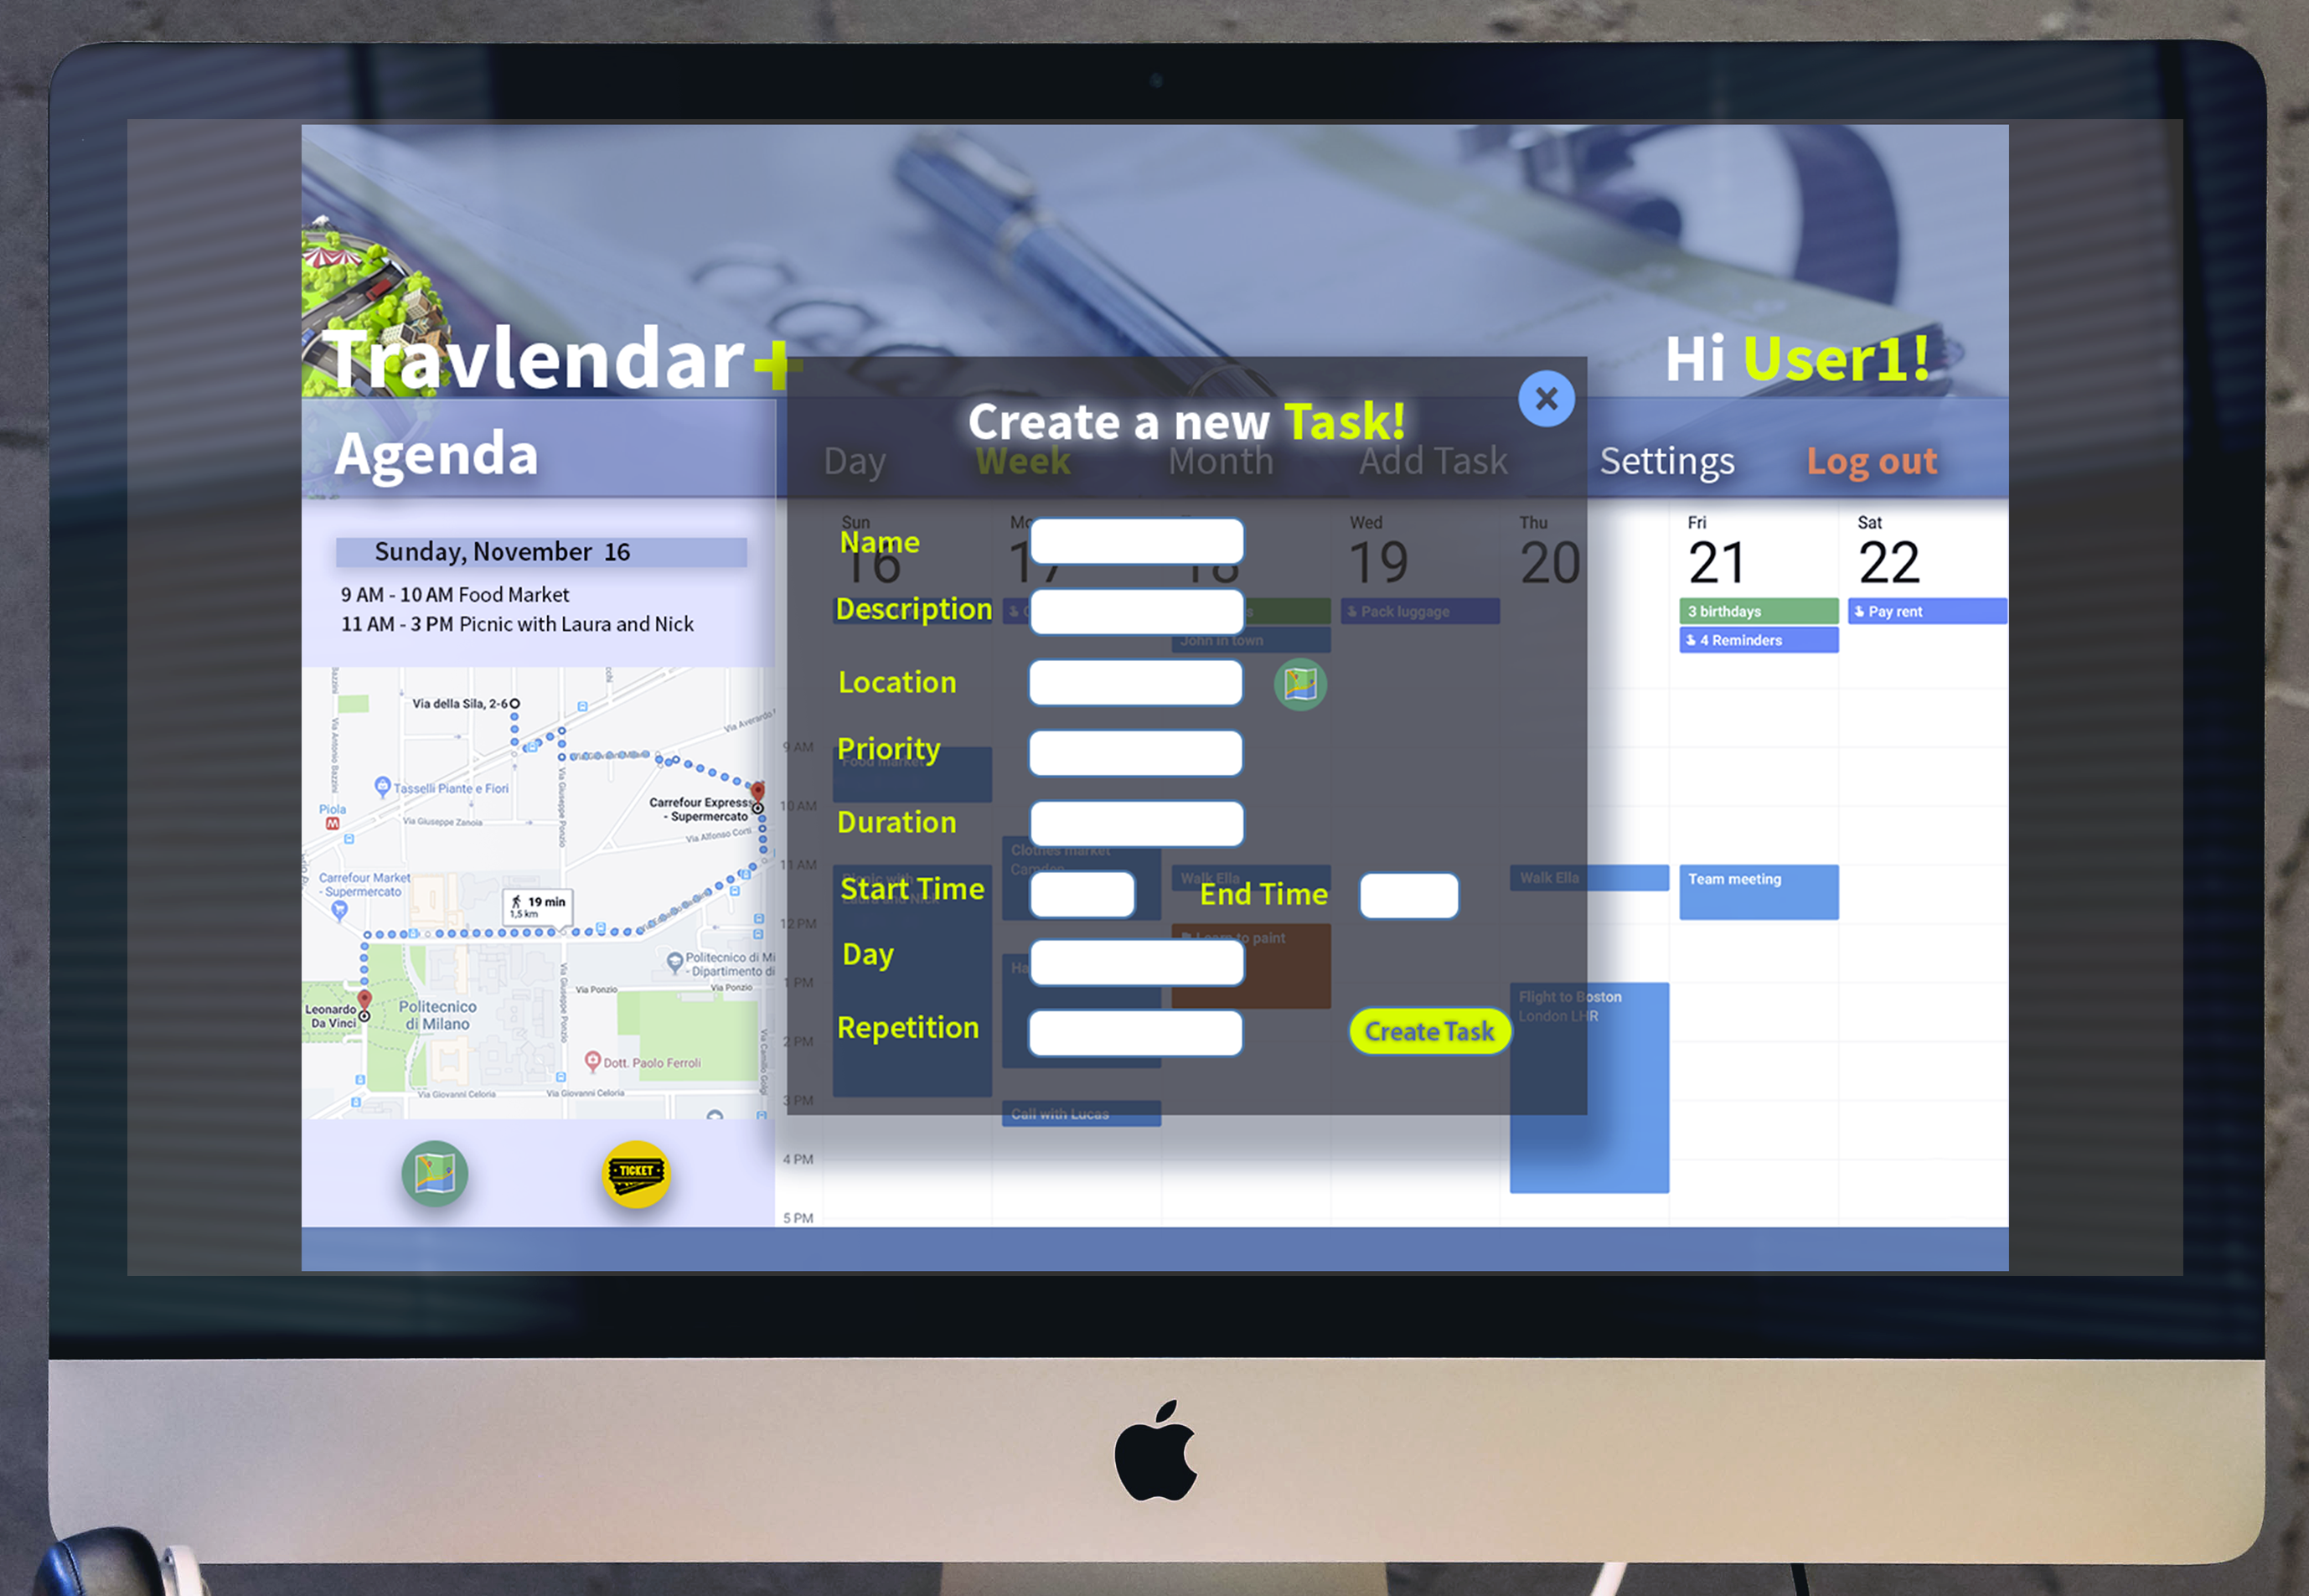
\includegraphics[scale=0.2]{Pictures/UXDiagram/desktopMockUpAddTask.png}
    \caption{Mock Up for the creation of a new task}
    \label{fig:addTaskMockUp}
=======
    \label{fig:my_label}
>>>>>>> ad258dd7c9a37861a484c05c0be22fc9761a519f
\end{figure}